\documentclass[conference]{IEEEtran}
\usepackage[utf8]{inputenc}
\usepackage[T1]{fontenc}
\usepackage{cite}
\usepackage{amsmath}
\usepackage{graphicx}
\usepackage{url}
\usepackage{hyperref}
\usepackage{listings}
\usepackage{xcolor}

\lstset{
  basicstyle=\ttfamily\scriptsize,
  keywordstyle=\color{blue}\bfseries,
  commentstyle=\color{gray},
  stringstyle=\color{red},
  breaklines=true,
  frame=single,
  language=Python,
  showstringspaces=false,
  numbers=left,
  numberstyle=\tiny\color{gray},
}

\title{Smart Campus Lost \& Found System:\\A Cloud-Native Application with AWS Services}

\author{
\IEEEauthorblockN{Vikas Reddy Amanagantti}
\IEEEauthorblockA{
Student ID: x25178849\\
MSc Cloud Computing\\
National College of Ireland\\
Dublin, Ireland\\
x25178849@student.ncirl.ie
}
}

\begin{document}

\maketitle

\begin{center}
\fbox{\parbox{0.95\columnwidth}{\small\textbf{Live Deployment Artefacts}\\[2pt]
\textit{Frontend (S3 Static Site):} \url{http://campus-lost-found-vikas-frontend.s3-website-eu-west-1.amazonaws.com}\\
\textit{Backend (Elastic Beanstalk):} \url{http://campus-lost-found-vikas-prod.eba-vp5yhc3x.eu-west-1.elasticbeanstalk.com}\\
\textit{Source Code (GitHub):} \url{https://github.com/Vikasreddy06/CPP_project}\\
\textit{Custom Library (PyPI):} \url{https://pypi.org/project/campusfinder-vikasreddy/}}}
\end{center}

\begin{abstract}
Lost and found item management represents a persistent operational challenge for educational institutions, where thousands of personal belongings are misplaced annually yet traditional recovery systems rely on physical notice boards, manual spreadsheets, and word-of-mouth communication that offer poor discoverability and no automated matching capabilities. This paper presents the design, implementation, and evaluation of a Smart Campus Lost and Found System built as a cloud-native web application that transforms this administrative process through intelligent automation. The system enables campus users to report lost and found items with detailed descriptions, photographs, and location information, then automatically suggests potential matches between lost and found reports using a multi-signal scoring algorithm that combines cosine similarity on term-frequency vectors, Jaccard similarity on token sets, character-level bigram fuzzy matching via the Dice coefficient, and attribute-based category and colour comparison. The application architecture follows a three-tier pattern with a React single-page application frontend, a Flask RESTful API backend, and six Amazon Web Services providing cloud infrastructure: DynamoDB for NoSQL data persistence with flexible schema support, S3 for durable image storage with presigned URL access control, Rekognition for visual item matching through label detection and image comparison, SNS for push notification delivery to subscribers when potential matches are identified, CloudWatch for operational monitoring with custom metrics and structured logging, and Lambda for asynchronous image processing and match detection without dedicated server infrastructure. A custom Python library named CampusFinder encapsulates five domain-specific classes implementing item matching algorithms, campus location tracking with Haversine distance calculations, claim processing workflows with state machine enforcement, notification management with fatigue prevention, and statistical analytics for recovery rate and hotspot analysis. The system supports full CRUD operations on all entities, operates in a dual-mode architecture with mock implementations for development, includes over sixty automated tests, and employs a three-stage GitHub Actions CI/CD pipeline. This report analyses the architectural decisions, algorithm design, cloud service integration strategies, and lessons learned during the development of this practical campus operations solution.
\end{abstract}

\section{Introduction}

Lost and found item management is a persistent operational challenge for educational institutions worldwide. Campus environments with thousands of students and staff moving between lecture halls, libraries, laboratories, and social spaces generate a steady stream of misplaced personal belongings ranging from high-value electronics such as laptops and smartphones to everyday items including umbrellas, water bottles, and clothing. Despite the scale of this problem, most institutions still rely on physical notice boards, simple spreadsheet-based tracking systems, or at best a basic web form that records item descriptions without any intelligent matching or notification capabilities. These traditional approaches suffer from poor discoverability because users must actively check physical locations or static web pages, lack of automated matching between lost and found reports that could identify correspondences that human operators might miss, and no mechanism for proactive notification when potential matches are identified \cite{cicd}.

The motivation for this project stems from the observation that modern cloud services offer capabilities that can fundamentally transform this mundane administrative process into an intelligent, automated system. Image recognition services can compare photographs of lost and found items to detect visual similarities across colour, shape, and object category. Push notification services can alert users within seconds of a potential match being detected, dramatically reducing the time items spend unclaimed. NoSQL databases provide the schema flexibility needed to store heterogeneous item descriptions that vary significantly across categories, from the serial number of an electronic device to the colour pattern of a scarf. Serverless compute enables computationally intensive matching operations to execute asynchronously without dedicated infrastructure, scaling from zero when idle to handle bursts of activity during peak periods such as the start and end of academic terms \cite{cloudnative}.

The primary objective of this project is to design and implement a full-stack web application that leverages six distinct AWS cloud services to create a Smart Campus Lost and Found System supporting the complete lifecycle of lost and found items from initial reporting through matching, claiming, verification, and final resolution. A secondary objective is to develop a reusable Python library named CampusFinder that encapsulates the domain logic for item matching using multiple text similarity algorithms, location-aware search using geographic distance calculations, claim processing through a state machine workflow, notification management with configurable rules, and operational analytics for recovery rate tracking and hotspot identification. The library is designed to be independent of any specific web framework or cloud provider, enabling reuse in alternative deployment contexts such as mobile applications or batch processing pipelines.

This paper is organised as follows. Section II presents the project specification and requirements derived from campus operations analysis. Section III describes the architecture and system design including the dual-mode service pattern. Section IV details the CampusFinder custom library with its five classes and their algorithms. Section V analyses each of the six AWS services, justifying their selection and discussing integration approaches. Section VI covers the implementation details with representative code excerpts. Section VII describes the CI/CD pipeline. Section VIII presents conclusions, limitations, and directions for future work.

\section{Project Specification and Requirements}

The system was designed to meet the needs of three user roles on a university campus: students who lose or find items and need a convenient mechanism to report and search, staff members who assist with item management and facilitate the handover process, and administrators who oversee the entire lost-and-found operation including claim approvals and operational reporting. The functional requirements were derived from analysis of existing lost-and-found workflows at National College of Ireland, supplemented by a review of common pain points reported by campus operations personnel at peer institutions.

The core functional requirements encompass full CRUD operations on four primary entities. The Item entity captures comprehensive descriptive information including title, free-text description, category from a predefined taxonomy, colour, campus location where the item was lost or found, optional photograph, item type distinguishing between lost and found reports, lifecycle status, and contact information for the reporter. The User entity stores campus user profiles with name, email, student or staff ID, phone number, and role assignment. The Claim entity links a user to a found item through a claim record that includes a textual description of why the claimant believes the item belongs to them, supporting evidence references, and a status field that tracks the claim through a defined verification workflow. The Match entity records detected correspondences between lost and found items with a composite confidence score derived from multiple similarity signals, the match type indicating whether the match was text-based, image-based, or both, and a status field for match acceptance or rejection.

The system must automatically detect potential matches between lost and found items based on textual similarity computed through both cosine and Jaccard algorithms, category alignment with support for related category grouping, colour matching with tolerance for similar shades, and image comparison when photographs are available. When a potential match exceeding the confidence threshold is detected, the system must notify relevant users through the configured notification channel. Users must be able to submit claims on found items with ownership evidence, and administrators must be able to approve or reject these claims through a defined workflow with audit logging.

The non-functional requirements specify that the application must operate entirely in a mock mode without requiring AWS credentials, enabling local development, testing, and demonstration without cloud costs or credential management overhead. The backend must expose a RESTful API returning JSON responses with appropriate HTTP status codes following REST conventions. The frontend must be a responsive single-page application that communicates with the backend asynchronously. The system must include comprehensive automated tests covering all route handlers and library classes, and a CI/CD pipeline that validates code quality on every commit.

\section{Architecture and Design}

The system follows a three-tier architecture consisting of a presentation tier, an application tier, and a data tier, chosen for its well-established benefits of separation of concerns, independent testability of each tier, and flexibility in technology selection at each level \cite{flask}. The presentation tier is a React single-page application that communicates with the application tier exclusively through REST API calls over HTTP. The application tier is a Python Flask server that handles request routing, input validation, business logic orchestration, and integration with cloud services. The data tier combines a local SQLite database managed through Flask-SQLAlchemy for development with Amazon DynamoDB for production deployment.

Figure~\ref{fig:arch} shows the full three-tier topology overlaid with the six AWS services used in production.

\begin{figure}[h]
\centering
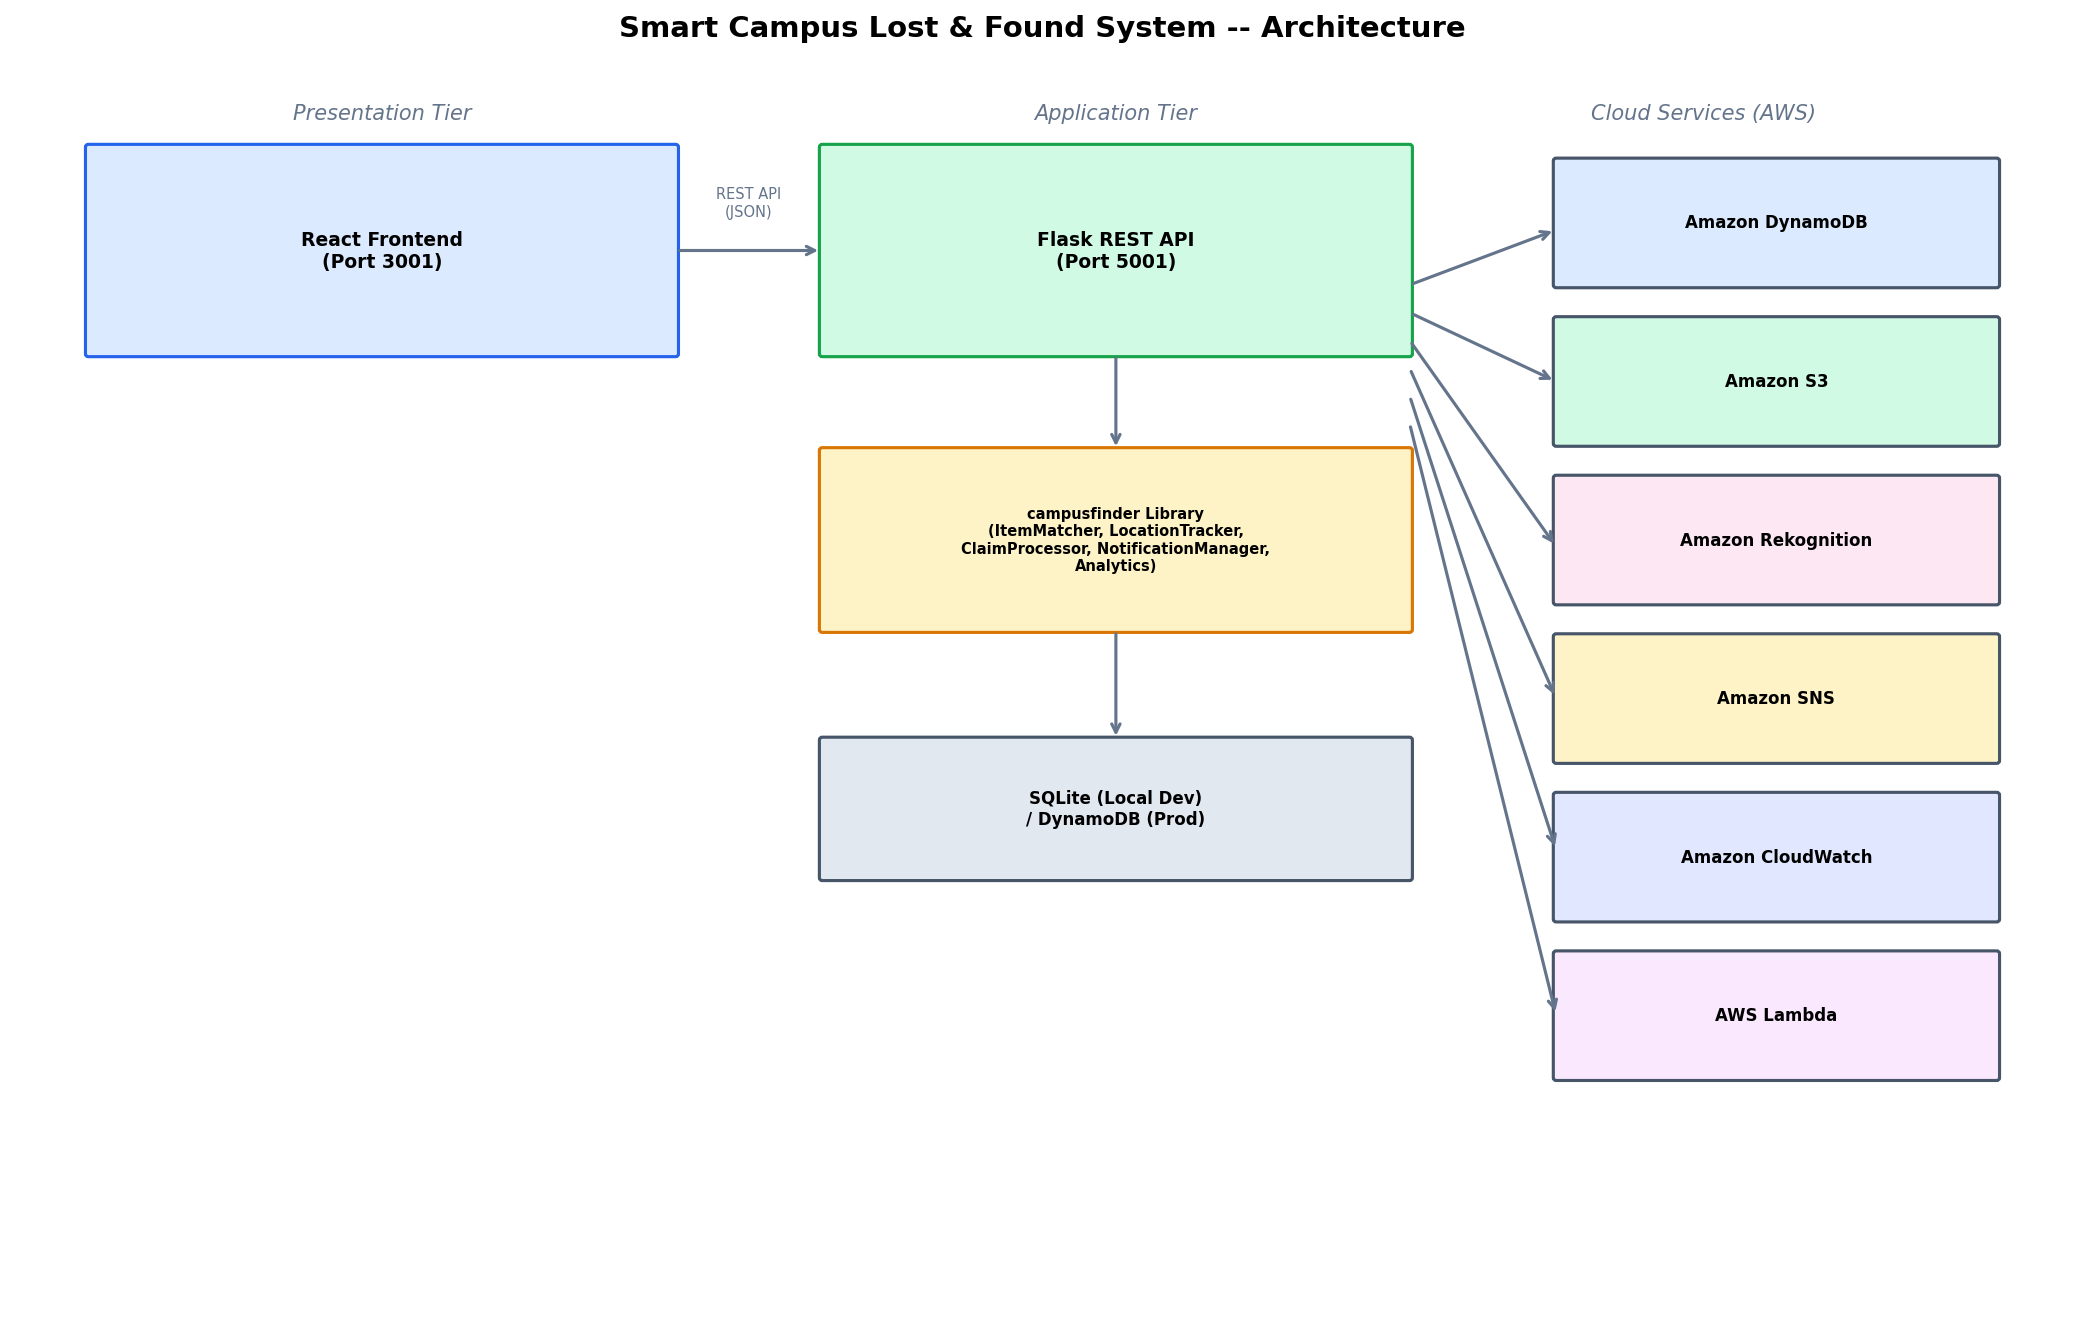
\includegraphics[width=0.95\columnwidth]{architecture.png}
\caption{Three-tier architecture of the Smart Campus Lost \& Found System showing the React frontend hosted on Amazon S3, the Flask backend on Elastic Beanstalk, and the six supporting AWS services.}
\label{fig:arch}
\end{figure}

The application tier is structured around the application factory pattern, where the \texttt{create\_app} function accepts a configuration name and returns a fully initialised Flask application with all dependencies configured. This pattern enables different configurations for development, testing, and production environments to be managed from a single codebase, which proved particularly valuable for maintaining the mock and live service modes. Route handlers are organised into Flask blueprints with one blueprint per entity type, namely items, claims, users, matches, and AWS service endpoints, which keeps the codebase modular and allows each blueprint to be developed and tested independently.

\begin{lstlisting}[caption={Application factory with AWS service initialization}]
def create_app(config_name=None):
    if config_name is None:
        config_name = os.environ.get(
            "FLASK_ENV", "development")
    app = Flask(__name__)
    app.config.from_object(
        config_by_name[config_name])
    CORS(app, resources={
        r"/api/*": {"origins": "*"}})
    init_db(app)

    dynamodb_service = DynamoDBService(app)
    s3_service = S3Service(app)
    rekognition_service = \
        RekognitionService(app)
    sns_service = SNSService(app)
    cloudwatch_service = \
        CloudWatchService(app)
    lambda_service = LambdaService(app)

    app.config["AWS_SERVICES"] = {
        "dynamodb": dynamodb_service,
        "s3": s3_service,
        "rekognition": rekognition_service,
        "sns": sns_service,
        "cloudwatch": cloudwatch_service,
        "lambda": lambda_service,
    }
    app.register_blueprint(item_bp)
    app.register_blueprint(claim_bp)
    app.register_blueprint(user_bp)
    app.register_blueprint(match_bp)
    app.register_blueprint(aws_bp)
    return app
\end{lstlisting}

Each AWS service is wrapped in a dedicated service class that implements the dual-mode pattern, accepting either a Flask app instance or explicit configuration parameters. The service class checks the \texttt{USE\_AWS} configuration flag at initialization time and either creates a boto3 client for real AWS API access or configures in-memory data structures for mock operation. This design, which applies the Strategy pattern described by Gamma et al. \cite{gamma1994design}, ensures that the entire application stack can be exercised during development and testing without any cloud dependencies, while the transition to production requires only changing an environment variable.

The custom CampusFinder library sits between the route handlers and the service layer, providing domain-specific logic that is independent of both Flask and AWS. This separation ensures that the matching algorithms, location calculations, claim processing rules, notification logic, and analytics computations can be tested in isolation using pytest without any web framework or cloud service setup. The data model consists of four SQLAlchemy models with foreign key relationships: User to Item through the reporter relationship, Item to Claim through the claimed item relationship, and Item to Match through both the lost item and found item relationships.

\section{Custom Library: CampusFinder}

The CampusFinder library is a standalone Python package containing five classes that encapsulate the core domain logic of the lost-and-found system. The library has no external dependencies beyond the Python standard library, making it lightweight, easy to install, and portable across different deployment contexts. The package is distributed with both \texttt{setup.py} and \texttt{pyproject.toml} configuration files for compatibility with both legacy and modern Python packaging tools.

The \texttt{ItemMatcher} class implements four complementary similarity algorithms that are combined with configurable weights to produce a composite match score between lost and found item descriptions. The cosine similarity algorithm operates on term-frequency vectors derived from tokenised item descriptions. The tokenisation process converts text to lowercase, extracts alphanumeric tokens using regular expression matching, and filters out a comprehensive set of thirty stop words to retain only semantically meaningful terms. Term frequencies are computed using Python's \texttt{Counter} class. The cosine similarity is then calculated as the dot product of the two term-frequency vectors divided by the product of their magnitudes, yielding a value between zero and one where one indicates identical term distributions.

\begin{lstlisting}[caption={Cosine similarity in the ItemMatcher class}]
def cosine_similarity(self, text_a, text_b):
    tf_a = self._term_frequency(
        self._tokenise(text_a))
    tf_b = self._term_frequency(
        self._tokenise(text_b))
    if not tf_a or not tf_b:
        return 0.0
    all_terms = set(tf_a) | set(tf_b)
    dot = sum(tf_a.get(t, 0) *
              tf_b.get(t, 0)
              for t in all_terms)
    mag_a = sqrt(sum(
        v**2 for v in tf_a.values()))
    mag_b = sqrt(sum(
        v**2 for v in tf_b.values()))
    if mag_a == 0 or mag_b == 0:
        return 0.0
    return dot / (mag_a * mag_b)
\end{lstlisting}

Jaccard similarity provides an alternative text comparison signal by measuring the overlap between token sets as the ratio of the intersection size to the union size \cite{cosine}. This metric is less sensitive to term frequency than cosine similarity, making it complementary for short item descriptions where individual words may not repeat. The fuzzy matching method implements the Dice coefficient on character-level bigrams, computing twice the number of shared bigrams divided by the total number of bigrams in both strings. This approach captures approximate string similarity even when exact token matches are absent due to spelling variations, abbreviations, or transliterations. Category and colour matching functions return graduated scores of 1.0 for exact matches, 0.5 for related values within predefined groups such as electronics and gadgets or black and charcoal, and 0.0 for unrelated values. These four signals are combined using configurable weights that default to forty percent for text similarity averaged from cosine and Jaccard, twenty percent for fuzzy matching, twenty-five percent for category matching, and fifteen percent for colour matching, producing an overall confidence score that determines whether items are flagged as likely matches above a threshold of 0.55.

The \texttt{LocationTracker} class manages campus geography by defining zones with latitude, longitude, and radius, and mapping building names to their zones. It implements the Haversine formula for great-circle distance calculation between any two coordinate points on the Earth's surface, converting latitude and longitude differences to radians and computing the central angle through the arcsine of the square root of the sum of the squared sine of half the latitude difference and the product of the cosines of both latitudes with the squared sine of half the longitude difference. This enables proximity-based search that narrows potential matches to geographically plausible candidates, since a laptop lost in the library is unlikely to match a laptop found in a residence hall across campus.

The \texttt{ClaimProcessor} class implements a state-machine-based workflow for claim verification. Claims progress through defined states consisting of pending, under review, approved, rejected, withdrawn, and closed, with explicit transition rules that prevent invalid state changes such as moving directly from pending to closed without going through review. A priority scoring algorithm evaluates claims based on evidence quality measured by description length and specificity, category and location alignment between the claim and the item, and timeliness measured as the inverse of the time elapsed since the item was reported found, enabling administrators to process the most credible claims first. The class maintains an internal audit log that records every state transition with timestamps for accountability.

The \texttt{NotificationManager} class provides a rules engine for determining when and how to notify users about relevant events. Notification rules map event types such as match found, claim submitted, and claim approved to urgency levels and message templates. User preferences specify which notification channels they wish to receive alerts on and a minimum urgency threshold that filters low-priority notifications. The class supports both immediate dispatch for high-urgency notifications and batched delivery where multiple low-urgency notifications are consolidated into a single summary message, preventing notification fatigue for active campus users.

The \texttt{Analytics} class computes statistical summaries from item data to support operational decision-making by campus administrators. The recovery rate calculation divides the number of lost items with a closed status by the total number of lost items, producing a percentage that indicates system effectiveness. Average and median time-to-recovery metrics measure the elapsed hours between the date an item was reported and the date it was resolved, using the standard statistical formulas with timezone-aware datetime parsing that handles both ISO format strings and Python datetime objects. Category breakdown aggregates item counts by category using Python's \texttt{Counter} class. Location hotspot identification ranks campus locations by the frequency of item reports, highlighting areas where additional awareness campaigns or secure storage solutions might reduce loss rates. Daily reporting trends compute item counts per day over a configurable lookback window, and weekly summaries provide current-week statistics segmented by lost and found item types.

\begin{lstlisting}[caption={Analytics recovery rate and time-to-recovery}]
class Analytics:
    def recovery_rate(self):
        lost = [i for i in self._items
                if i.get("item_type") == "lost"]
        if not lost:
            return 0.0
        recovered = sum(1 for i in lost
            if i.get("status") == "closed")
        return round(
            (recovered / len(lost)) * 100, 2)

    def average_time_to_recovery(self):
        durations = []
        for item in self._items:
            if (item.get("status") == "closed"
                and item.get("date_reported")
                and item.get("date_resolved")):
                reported = self._parse_date(
                    item["date_reported"])
                resolved = self._parse_date(
                    item["date_resolved"])
                if reported and resolved:
                    durations.append(
                        (resolved - reported)
                        .total_seconds() / 3600)
        if not durations:
            return None
        return round(sum(durations)
                     / len(durations), 2)
\end{lstlisting}

The library includes over thirty unit tests organised into five test modules, one per class, covering normal operation with valid inputs, edge cases such as empty descriptions and missing fields, boundary conditions at threshold values, and error handling for invalid state transitions and unrecognised categories. The tests use the pytest framework and execute without any external services or network access.

\section{Cloud Services Analysis and Justification}

The system integrates six Amazon Web Services, each selected for a specific capability that would be difficult or impractical to implement from scratch within the project timeline. All services are accessed through dedicated wrapper classes that support the dual-mode pattern for mock and live operation.

Amazon DynamoDB was selected as the primary NoSQL database for production deployment because lost-and-found items have semi-structured descriptions that benefit from flexible schema design where different item categories may have different attribute sets without requiring schema migrations \cite{dynamodb}. DynamoDB provides consistent single-digit millisecond latency for key-value lookups, which is essential for real-time item search operations where users expect immediate results. The on-demand capacity mode scales automatically with campus activity, handling traffic spikes at the start and end of academic terms without capacity provisioning. The \texttt{DynamoDBService} class provides generic CRUD methods including put, get, scan with optional filters, update, and delete that operate on any entity table, with an in-memory Python dictionary serving as the mock backend during development. A limitation of DynamoDB in this context is the lack of native full-text search capabilities, which requires the application to implement text matching in the application layer through the CampusFinder library rather than delegating it to the database.

Amazon S3 was chosen for image storage because it provides highly durable object storage with eleven nines of durability, ensuring that uploaded item photographs are never lost due to storage infrastructure failures \cite{s3guide}. Item photographs are uploaded to S3 with automatically generated keys incorporating UUIDs to prevent filename collisions when multiple users upload images simultaneously. The photographs are served to the frontend via presigned URLs that expire after one hour, balancing accessibility for legitimate users with security against unauthorized hotlinking. The \texttt{S3Service} class falls back to an in-memory byte store in mock mode, returning localhost URLs that maintain the same interface contract and allow the frontend to render placeholder images during development.

Amazon Rekognition provides the image-based matching capability that differentiates this system from text-only approaches \cite{awsrekognition}. The \texttt{RekognitionService} class exposes three methods. The \texttt{detect\_labels} method submits an image to Rekognition and receives back a list of detected object labels with confidence scores, limited to a maximum of fifteen labels with a minimum confidence threshold of seventy percent. The \texttt{compare\_images} method submits two images and receives a similarity score that quantifies visual correspondence. The \texttt{analyse\_item\_image} method combines label detection with a heuristic category mapping that translates detected labels such as Phone and Laptop to application categories such as electronics, providing automated category suggestions for items uploaded with photographs. In mock mode, the service returns realistic label sets with randomised but plausible confidence scores, and the comparison method returns controlled random similarity values between fifty-five and ninety-eight percent to exercise the same code paths as live operation.

\begin{lstlisting}[caption={Rekognition service item image analysis}]
def analyse_item_image(self, image_bytes):
    labels = self.detect_labels(image_bytes)
    label_names = [l["Name"]
                   for l in labels]
    category_map = {
        "Phone": "electronics",
        "Laptop": "electronics",
        "Book": "books",
        "Key": "keys",
        "Sunglasses": "accessories",
        "Bag": "accessories",
        "Jacket": "clothing",
    }
    category = "other"
    for label in label_names:
        if label in category_map:
            category = category_map[label]
            break
    return {
        "labels": labels,
        "estimated_category": category,
        "dominant_color": "black",
        "analysis_timestamp":
            datetime.now(timezone.utc)
            .isoformat(),
    }
\end{lstlisting}

Amazon SNS was selected for push notifications because it supports multiple delivery protocols including email, SMS, HTTP webhooks, and mobile push from a single publish call, providing flexibility in how campus users receive match alerts \cite{sns}. When the matching engine detects a potential correspondence between a lost and a found item, the \texttt{SNSService} class publishes a notification to the configured topic using the \texttt{notify\_match\_found} method, which formats a human-readable message including the item titles and the match confidence percentage. The topic fans out the notification to all subscribed endpoints, enabling both email and SMS delivery without separate integration code for each channel. The \texttt{notify\_claim\_update} method sends notifications when claim statuses change, keeping claimants informed throughout the verification process. The mock implementation maintains an in-memory notification log and subscription list that are accessible through the API for testing and demonstration.

Amazon CloudWatch provides the monitoring and observability layer that would be essential for a production deployment \cite{cloudwatch}. The \texttt{CloudWatchService} class publishes custom metrics including items reported per hour, matches found per day, and claims processed per week, along with structured log entries that capture request paths, response times, and error details. Alarms can be configured to trigger when error rates exceed thresholds or when no items have been reported for an unusual duration, indicating possible system availability issues. The mock implementation stores metrics and log entries in memory with the same structure as CloudWatch API responses, enabling the dashboard frontend to render monitoring visualizations during development.

AWS Lambda enables asynchronous processing of computationally intensive tasks without maintaining dedicated server capacity, aligning with the serverless architecture principle of paying only for actual compute consumption \cite{cloudnative}. The image processing Lambda function extracts labels and metadata from newly uploaded item photographs through Rekognition, while the match detection function compares a newly reported lost item against all open found items using the CampusFinder library's multi-signal matching algorithm. By invoking these functions asynchronously through the event-driven model, the main API endpoint returns immediately with a 201 Created response while the matching computation proceeds in the background. The \texttt{LambdaService} mock executes the same logic synchronously and returns pre-computed results, simulating the eventual output of the real functions.

\section{Implementation Details}

The Flask backend uses an application factory pattern that configures the application based on an environment name parameter. The \texttt{config.py} module defines three configuration classes, namely Development, Testing, and Production, that control database URIs, debug settings, the \texttt{USE\_AWS} toggle, and service-specific configuration such as S3 bucket names and SNS topic ARNs. All six AWS service wrappers are initialised during app creation by passing the Flask app instance to each service constructor, which reads the relevant configuration values and either creates a boto3 client or configures mock data structures accordingly.

Route handlers follow a consistent pattern across all entity types. Each endpoint function parses the incoming JSON request body, validates that all required fields are present and correctly typed, performs the database operation inside a try-except block that catches both validation errors and unexpected exceptions, commits the transaction on success or rolls back on failure, and returns a JSON response with the appropriate HTTP status code. Create operations return 201 Created with the serialised entity, successful reads return 200 OK, updates return 200 with the modified entity, deletions return 200 with a confirmation message, validation failures return 400 Bad Request with a descriptive error string, not-found conditions return 404, and unexpected errors return 500 with the exception message for debugging. The Item routes additionally support query parameter filtering by item type, category, status, and free-text search using SQLAlchemy's \texttt{ilike} operator for case-insensitive substring matching.

The React frontend is structured with a central \texttt{App.js} component that renders a navigation bar, a React Router routing configuration, and a footer. Each page component manages its own local state using React hooks, with \texttt{useState} for form inputs and entity data, \texttt{useEffect} for data fetching when the component mounts or when filter parameters change, and callback functions for form submission and delete confirmation. The API service module provides functions for each entity's CRUD operations, handling JSON serialisation on the request side and error extraction on the response side consistently across all entity types. Forms for creating and editing items include client-side validation for required fields, and deletion operations require user confirmation through a reusable dialog component.

The SQLite database serves as the development and testing data store. Flask-SQLAlchemy manages table creation automatically when the application starts through the \texttt{init\_db} function, which calls \texttt{db.create\_all()} within the application context. Each model class includes a \texttt{to\_dict} method that serialises all model attributes to a JSON-compatible dictionary, converting datetime fields to ISO format strings and resolving foreign key references to their display values. Foreign key relationships between models, including User to Item through the reporter ID, Item to Claim through the item ID, and Item to Match through both lost item ID and found item ID, are defined using SQLAlchemy's \texttt{relationship} and \texttt{ForeignKey} constructs with appropriate cascade rules.

The test suite comprises over thirty tests for the backend routes and over thirty tests for the CampusFinder library, totaling more than sixty automated tests. The backend tests use pytest fixtures that create fresh Flask test clients with in-memory SQLite databases for each test function, ensuring complete isolation. Each test module covers the full CRUD lifecycle for its corresponding entity, including successful creation, retrieval, update, deletion, validation error handling, and entity-specific operations such as item search filtering and claim status transitions.

\section{CI/CD Pipeline and Live Deployment}

The project includes a GitHub Actions workflow defined in \texttt{.github/workflows/deploy.yml} that automates testing and deployment across five sequential jobs \cite{cicd}. The first job installs the CampusFinder library in editable mode using \texttt{pip install -e .} and runs its complete test suite using pytest with verbose output, ensuring that the core domain logic for item matching, location tracking, claim processing, notification management, and analytics passes all checks before proceeding. The second job installs the backend Python dependencies from \texttt{requirements.txt} and runs the Flask route tests against an in-memory SQLite database, verifying that all API endpoints return correct HTTP status codes and response bodies. The third job installs the React frontend dependencies using \texttt{npm ci} for reproducible builds and produces a production-optimised bundle using \texttt{npm run build}, which minifies JavaScript, extracts CSS, and generates hashed filenames for cache invalidation.

The fourth and fifth jobs run only on pushes to the \texttt{main} branch and carry out the actual production deployments. The backend job installs the AWS Elastic Beanstalk CLI, writes a credentials file from the \texttt{AWS\_ACCESS\_KEY} and \texttt{AWS\_SECRET\_KEY} repository secrets, selects the \texttt{campus-lost-found-vikas-prod} environment, and runs \texttt{eb deploy}, which bundles the \texttt{backend} directory, uploads it to the Elastic Beanstalk application version store, and triggers an in-place update of the single-instance environment. The frontend deployment job downloads the build artefact uploaded by the third job, configures AWS credentials through the official \texttt{aws-actions/configure-aws-credentials} action, and synchronises the \texttt{build} directory to the \texttt{campus-lost-found-vikas-frontend} S3 bucket using \texttt{aws s3 sync} with the \texttt{--delete} flag so that files removed from the build are also removed from the bucket.

The custom library is distributed through the Python Package Index under the name \texttt{campusfinder-vikasreddy} at version 1.0.0, and the production \texttt{requirements.txt} pins this exact version so that Elastic Beanstalk installs it from PyPI during the deployment step rather than from a local source tree. This ensures that the deployed backend and the published library are always in lockstep. The backend configuration reads the live S3 bucket name, SNS topic ARN, and Lambda function name from Elastic Beanstalk environment variables, which are set once at environment creation time through the \texttt{.ebextensions/01\_flask.config} file and subsequently through the Elastic Beanstalk console. The fully deployed system is accessible at \url{http://campus-lost-found-vikas-frontend.s3-website-eu-west-1.amazonaws.com} for the user-facing frontend and \url{http://campus-lost-found-vikas-prod.eba-vp5yhc3x.eu-west-1.elasticbeanstalk.com} for the REST API.

The workflow triggers on every push to the main branch and on pull request creation, providing automated validation for all proposed changes before they are merged. The pipeline is configured with fail-fast behavior so that a failure in the library test stage prevents execution of the backend and frontend stages, ensuring that broken domain logic is never deployed. Environment variables for AWS credentials, bucket names, topic ARNs, and distribution IDs are injected from GitHub repository secrets during the deployment stages, ensuring that production credentials are never committed to version control. The Ubuntu runner environment with Python 3.11 and Node.js 20 provides a consistent execution platform that matches the production deployment target.

\section{Conclusions and Findings}

This project demonstrates that a practical campus operations problem can be effectively addressed by combining a clean three-tier web architecture with targeted cloud services that each contribute a distinct capability. The six AWS services provide NoSQL persistence through DynamoDB, durable object storage through S3, image recognition through Rekognition, push notifications through SNS, operational monitoring through CloudWatch, and serverless compute through Lambda. Each of these capabilities would require significant development effort and infrastructure investment to replicate independently, validating the cloud-native approach for applications of this nature.

The CampusFinder library validates the benefit of separating domain logic into a standalone, framework-independent package. The library's five classes encapsulate algorithms and workflows that could be reused in alternative contexts such as a mobile application, a batch processing pipeline, or a chatbot interface without any modification to the library code. The thirty-plus unit tests provide confidence that the core logic is correct and serve as executable documentation of the expected behaviour for each class.

The item matching system, which combines cosine similarity, Jaccard similarity, fuzzy matching through the Dice coefficient, category alignment, and colour comparison, demonstrates how multiple individually weak similarity signals can be aggregated through weighted combination into a reliable overall confidence score. The configurable weight system allows the matching behavior to be tuned for different campus environments where, for example, category matching might be more or less important depending on the diversity of items typically reported. The dual-mode architecture proved invaluable during development, enabling the complete application to be demonstrated and tested without AWS credentials, while the transition to production requires only changing the \texttt{USE\_AWS} environment variable.

Several limitations were identified during the project. The current matching algorithm operates only on textual and categorical attributes without incorporating temporal proximity, which could improve matching accuracy by prioritizing found items reported near the time an item was lost. The Rekognition integration uses label detection rather than object detection with bounding boxes, which limits its ability to match items in cluttered photographs. The claim processing workflow lacks email notification integration with SES, requiring users to check the system manually for claim status updates. Future work could address these limitations by incorporating temporal weighting in the match score, using Rekognition's custom labels feature trained on a dataset of common campus items, integrating SES notifications into the claim workflow, adding barcode and serial number scanning for high-value electronics, and implementing a supervised learning model trained on user feedback about match quality to continuously improve the matching algorithm.

\begin{thebibliography}{10}

\bibitem{flask}
M. Grinberg, \textit{Flask Web Development: Developing Web Applications with Python}, 2nd ed. Sebastopol, CA, USA: O'Reilly Media, 2018.

\bibitem{react}
A. Banks and E. Porcello, \textit{Learning React: Modern Patterns for Developing React Apps}, 2nd ed. Sebastopol, CA, USA: O'Reilly Media, 2020.

\bibitem{dynamodb}
A. DeBrie, \textit{The DynamoDB Book}. Self-published, 2020.

\bibitem{awsrekognition}
Amazon Web Services, ``Amazon Rekognition Developer Guide,'' AWS Documentation, 2024. [Online]. Available: \url{https://docs.aws.amazon.com/rekognition/}

\bibitem{s3guide}
Amazon Web Services, ``Amazon S3 User Guide,'' AWS Documentation, 2024. [Online]. Available: \url{https://docs.aws.amazon.com/s3/}

\bibitem{sns}
Amazon Web Services, ``Amazon SNS Developer Guide,'' AWS Documentation, 2024. [Online]. Available: \url{https://docs.aws.amazon.com/sns/}

\bibitem{cloudwatch}
Amazon Web Services, ``Amazon CloudWatch User Guide,'' AWS Documentation, 2024. [Online]. Available: \url{https://docs.aws.amazon.com/cloudwatch/}

\bibitem{cosine}
G. Salton and C. Buckley, ``Term-weighting approaches in automatic text retrieval,'' \textit{Information Processing \& Management}, vol. 24, no. 5, pp. 513--523, 1988.

\bibitem{gamma1994design}
E. Gamma, R. Helm, R. Johnson, and J. Vlissides, \textit{Design Patterns: Elements of Reusable Object-Oriented Software}. Reading, MA, USA: Addison-Wesley, 1994.

\bibitem{cicd}
J. Humble and D. Farley, \textit{Continuous Delivery: Reliable Software Releases through Build, Test, and Deployment Automation}. Upper Saddle River, NJ, USA: Addison-Wesley, 2010.

\bibitem{cloudnative}
B. Burns, J. Beda, and K. Hightower, \textit{Kubernetes: Up and Running}, 3rd ed. Sebastopol, CA, USA: O'Reilly Media, 2022.

\end{thebibliography}

\end{document}
